\documentclass[11pt]{article}

\usepackage[margin=1in]{geometry}
\usepackage{amsmath,amssymb}
\usepackage{booktabs}
\usepackage{graphicx}
\usepackage{subcaption}
\usepackage{xcolor}
\usepackage{listings}
\usepackage{enumitem}
\usepackage[hidelinks]{hyperref}

\graphicspath{{../results/plots/}}
\setlist{itemsep=2pt, topsep=4pt}
\lstset{basicstyle=\ttfamily\small, breaklines=true, frame=single, columns=fullflexible,
        backgroundcolor=\color{gray!6}, rulecolor=\color{gray!40}}
\newcommand{\code}[1]{\texttt{#1}}
\newcommand{\pfp}{p_{\mathrm{fp}}}

\title{Bloom-Filter Context Compression for LLM Question Answering}
\author{COMP 580: Assignment 1, Swaha Roy}
\date{October 2026}

\begin{document}
\maketitle

\begin{abstract}
We compress long LLM contexts with a single, context-independent Bloom filter that stores a fixed
vocabulary of low-meaning English words and decorative markdown tokens. Compression is one pass
over the context: we split it into whitespace tokens (maximal runs of characters between spaces,
tabs or line breaks, so a word together with any punctuation attached to it) and drop every token
that the filter reports as present. With
\code{gemini-3.5-flash-lite} on the 80 questions of the four v1 contexts, our smallest vocabulary
(\code{curated}, 120 words, a 2{,}048-bit filter) cuts total LLM input tokens by 27\%
(2.66M $\to$ 1.94M) while accuracy moves from 86.3\% to 82.5\%, a difference of three questions.
Larger vocabularies compress more but lose accuracy steadily, and
false positives are far more damaging per token saved than deliberate removal. 
In Section 1, we introduce our implementation. In Section 2, we describe the experimental setup and metrics. 
In Section 3, we present our results. In Section 4, we answer the assignment questions.
\end{abstract}

% =========================================================================== %
\section{Context Compression via Bloom Filters}
\label{sec:method}
% =========================================================================== %

\subsection{Idea}
Long documents contain many words that carry little meaning on their own: \emph{the}, \emph{of},
\emph{was}, \emph{which}. They still cost input tokens. Our method stores a fixed vocabulary of such
words in \textbf{one} Bloom filter and deletes every context token that the filter matches:
\begin{align*}
\text{Baseline:}\quad & \mathrm{LLM}(\text{full context} + \text{question})\\
\text{Ours:}\quad & \text{full context} \xrightarrow{\ \text{one pass through the Bloom filter}\ }
  \text{compressed context} \xrightarrow{\ +\ \text{question}\ } \mathrm{LLM}
\end{align*}

We chose this design for three reasons.
\begin{itemize}
  \item \textbf{The Bloom filter \emph{is} the method.} Every removal decision is a membership
        query, so the filter parameters $R$ and $k$ have a direct, measurable effect on the output.
  \item \textbf{It is general.} The vocabulary is built only from fixed general-English lists. It
        never looks at the documents, questions or answers, so the identical filter is used on the
        held-out test contexts.
  \item \textbf{False positives have a visible cost.} A false positive deletes a word that is
        \emph{not} in the vocabulary, i.e.\ a content word such as a number, a name or a unit. The
        false-positive rate therefore translates directly into lost information, which makes the
        FPR--accuracy trade-off natural to study.
\end{itemize}

\subsection{Bloom filter implementation}
The filter is implemented from scratch in \code{ask\_llm.py} (class \code{BloomFilter}); only the
hash function comes from the standard library.
\begin{itemize}
  \item \textbf{Bit array.} A Python \code{bytearray} of $\lceil R/8\rceil$ bytes holds the $R$ bits.
  \item \textbf{Hashing.} Each word is hashed \emph{once} with keyed BLAKE2b
        (\code{hashlib.blake2b}, 16-byte digest, key = seed 580). The 128-bit digest is split into two
        64-bit integers $h_1$ and $h_2$; $h_2$ is forced odd. The $k$ bit positions come from
        Kirsch--Mitzenmacher double hashing:
        \[ g_i(x) = \bigl(h_1(x) + i\cdot h_2(x)\bigr) \bmod R, \qquad i = 0,\dots,k-1. \]
        A lookup therefore costs one hash call regardless of $k$, and the positions are identical
        across processes and machines. Python's salted built-in \code{hash()} is never used, because
        its value changes between runs.
  \item \textbf{Insert} sets the $k$ bits; \textbf{query} returns true only if all $k$ bits are set.
        There are no false negatives: every inserted word is always reported present (verified by
        unit tests).
  \item \textbf{Memoization.} The $(h_1,h_2)$ pair is cached per word (\code{functools.lru\_cache}),
        and compression memoizes the membership answer per distinct key, so each distinct word in a
        document is hashed once.
\end{itemize}
For $N$ inserted words the theoretical false-positive rate and the optimal number of hash functions
are
\[
  \pfp = \left(1 - e^{-kN/R}\right)^{k}, \qquad k_{\mathrm{opt}} = \frac{R}{N}\ln 2,
\]
and the number of bits needed for a target rate $p$ at $k_{\mathrm{opt}}$ is
\[
  R(p) = \left\lceil \frac{-N \ln p}{(\ln 2)^2} \right\rceil .
\]
In the code $k_{\mathrm{opt}}$ is rounded to the nearest integer and is at least 1.

\subsection{Vocabulary tiers}
The vocabulary is a second tuning knob beside $R$ and $k$. Every tier is built from fixed lists only:

\begin{table}[h]
\centering
\small
\begin{tabular}{@{}lp{9.6cm}r@{}}
\toprule
Tier & Contents & $N$ \\
\midrule
\code{curated} & NLTK's 179 English stopwords, minus the \emph{protected} words below, plus the
  decorative markdown tokens & 120 \\
\code{nltk\_full} & all 179 NLTK stopwords plus the decorative tokens (ablation: no protection) & 191 \\
\code{common500} & \code{curated} $\cup$ the 500 most frequent English words (\code{wordfreq} 3.1.1),
  ASCII letters only, protected words excluded & 464 \\
\code{common1000} & same, top 1{,}000 & 930 \\
\code{common2000} & same, top 2{,}000 & 1{,}905 \\
\code{common5000} & same, top 5{,}000 & 4{,}848 \\
\bottomrule
\end{tabular}
\caption{Vocabulary tiers. $N$ is the number of distinct words inserted into the filter.}
\label{tab:tiers}
\end{table}

\paragraph{Protected words.} Some stopwords can change or \emph{be} the answer to a question, so they
are never inserted into \code{curated} or the \code{common} tiers:
\begin{itemize}
  \item \textbf{negations} and their contraction stubs: \emph{no, nor, not, never, without, don't,
        isn't, wasn't, \dots} (and the stubs \emph{don, isn, wasn, \dots}) --- deleting \emph{not}
        inverts a fact;
  \item \textbf{comparatives and quantifiers}: \emph{more, most, less, least, few, only, same, very,
        than, all, any, each, both, some};
  \item \textbf{order and position words}: \emph{over, under, above, below, before, after, during,
        until, again};
  \item \textbf{single-letter fragments} that double as units or abbreviations: \emph{s, t, d, m, o,
        y, ll, re, ve, ma} (e.g.\ \emph{m} for meters, \emph{s} for seconds);
  \item \textbf{number and scale words} (\emph{zero}--\emph{ninety, hundred, thousand, million,
        billion, trillion, half, dozen}), \textbf{ordinals} \emph{first}--\emph{tenth},
        \textbf{months} and \textbf{weekdays}.
\end{itemize}

\paragraph{Decorative tokens.} \code{\#}, \code{\#\#}, \code{\#\#\#}, \code{\#\#\#\#}, \code{*},
\code{**}, \code{-}, \code{--}, \code{---}, \code{>}, \code{\textbullet}, \code{\_}. These are
markdown decoration that the model does not need. The table separator \code{|} is deliberately
\emph{not} removed, so table rows keep their column structure.

\subsection{Compression procedure}
\code{compress(text, bf)} makes a single pass over the context:
\begin{enumerate}
  \item Split each line on whitespace into \textbf{whitespace tokens}: maximal runs of
        non-whitespace characters, so \code{storm,} and \code{(the} are single tokens with their
        punctuation attached. Line breaks are kept (runs of blank lines are collapsed), so
        headings, list items and table rows stay on their own lines.
  \item For each token compute a \textbf{lookup key}: lowercase it, map the curly apostrophe
        (U+2019) to a straight one, and strip leading and trailing punctuation (\code{string.punctuation}
        plus curly quotes, en/em dashes and the ellipsis). If stripping leaves nothing (e.g.\ the
        token is \code{---}), the raw token is the key. Thus \code{The}, \code{the,} and \code{(the}
        all map to \code{the}.
  \item Drop the token if the key is in the filter; otherwise keep the \emph{original} token,
        including its punctuation and case.
\end{enumerate}
For example, with the \code{curated} filter,
\begin{lstlisting}
## Results
The mooring was moved to berths 9 through 17 after the storm, and it was not repaired until March.
\end{lstlisting}
becomes
\begin{lstlisting}
Results
mooring moved berths 9 17 after storm, not repaired until March.
\end{lstlisting}
The negation \emph{not}, the order words \emph{after}/\emph{until} and the month survive because
they are protected. The example also shows the method's main weakness: \emph{through} is a
stopword, but here it carries the meaning of a range.

Compressing a whole document (90--206\,KB) takes 10--35\,ms. The same filter is applied to every
context; the question and the instructions are never compressed, and neither are the model's
answers.

\subsection{Alternative approach: chunk-based retrieval}
The approach above was the second design we tried. Our first implementation was a chunk-based
retrieval design suggested by Claude, which worked as follows:
\begin{enumerate}
  \item Split the full context into chunks.
  \item For each chunk, extract several kinds of tokens from its text (e.g.\ words, word pairs and
        4-grams), and build one Bloom filter per chunk that stores them.
  \item At query time, tokenize the question the same way. For each chunk, check whether any of the
        question's tokens are present in that chunk's Bloom filter, and if so, add the chunk's text to
        the context.
\end{enumerate}
The compressed context therefore contains only the chunks that share at least one token with the
question.

We identified several shortcomings with this idea, and they motivated the redesign.
\begin{itemize}
  \item \textbf{A Bloom filter is not the right data structure here.} The filters depend on the full
        context, so we could simply use exact sets instead. A set has no false positives, so it would
        also compress the text more.
  \item \textbf{The memory saving does not matter.} Sets take more memory, but we already have to
        parse the full context and extract these tokens. The extra memory a set needs is therefore
        bounded by the size of the original context, up to constant factors.
  \item \textbf{There is no latency benefit.} In this setting the sets would not be stored on disk or
        in separate memory, so a set lookup is not meaningfully slower than a Bloom filter lookup.
\end{itemize}
So even if chunk-based retrieval compressed the context accurately, the case for using Bloom filters
to do it is not convincing.

The final design does not have this problem, because its filter holds a fixed vocabulary that does
not depend on any context. It could reasonably be built once offline and simply loaded at the start
of every question-answering call. Our implementation does build the filter from scratch at start-up,
but only because the assignment requires reproducible measurements; that constraint comes from the
assignment, not from the approach itself. Even so, the filter is built once at the start of each run
and reused across all contexts and questions.

\subsection{Hypotheses}
Before running the LLM experiments we expected:
\begin{enumerate}[label=\textbf{H\arabic*}]
  \item \textbf{FPR follows theory.} Because the hash positions are effectively uniform, the
        measured FPR should match $(1-e^{-kN/R})^k$ closely.
  \item \textbf{Tokens shrink less than words.} Stopwords are short and usually a single token,
        while the words that survive (numbers, names, units, punctuation) cost several tokens each.
        Removing $x\%$ of words should remove clearly less than $x\%$ of tokens.
  \item \textbf{A small, careful vocabulary stays close to the baseline.} The \code{curated} tier
        removes only function words that rarely carry facts, so accuracy should drop by only a few
        points. Larger tiers remove real content words (\emph{system, water, report, \dots}) and
        should lose accuracy steadily as $N$ grows.
  \item \textbf{False positives are worse than deliberate removal.} A false positive hits a
        \emph{random} non-vocabulary word, which is often exactly the number or name an answer needs.
        Per token saved, raising the FPR should cost much more accuracy than enlarging the vocabulary.
  \item \textbf{Memory has diminishing returns.} For a fixed vocabulary, once $R$ is large enough
        that $\pfp\approx 0$, more bits cannot change the compressed context, so token usage and
        accuracy should plateau.
\end{enumerate}

% =========================================================================== %
\section{Experimental Setup and Metrics}
\label{sec:setup}
% =========================================================================== %

\subsection{Data}
We use the four required v1 contexts and their 80 questions (20 per document). The answer files label
each question with a difficulty tier: 44 \textbf{T1} single-fact lookups, 24 \textbf{T2} multi-hop
questions and 12 \textbf{T3} aggregate questions (counting, summing or comparing across the
document).

\begin{table}[h]
\centering
\small
\begin{tabular}{@{}lrrrr@{}}
\toprule
Document & Words & Context tokens & Tokens after \code{curated} & Saved \\
\midrule
\code{antikythera\_dossier\_v1} & 21{,}156 & 32{,}764 & 24{,}888 & 24.0\% \\
\code{dwh\_dossier\_v1}         & 33{,}325 & 46{,}059 & 33{,}935 & 26.3\% \\
\code{harbour\_puzzle\_v1}      & 22{,}746 & 34{,}601 & 23{,}056 & 33.4\% \\
\code{lunarleaper\_2609\_11453} & 13{,}545 & 19{,}150 & 14{,}565 & 23.9\% \\
\midrule
Total & 90{,}772 & 132{,}574 & 96{,}444 & 27.3\% \\
\bottomrule
\end{tabular}
\caption{The four v1 contexts. Context tokens are Gemini tokens for the context alone.}
\label{tab:data}
\end{table}

\subsection{Fixed LLM setup}
Every run, baseline and compressed alike, uses the same model, prompt template and generation
configuration, so any difference is caused by the context alone.
\begin{itemize}
  \item \textbf{Model:} \code{gemini-3.5-flash-lite}, temperature 0, seed 580,
        \code{max\_output\_tokens} = 64. No thinking tokens were used (observed 0).
  \item \textbf{No system instruction.} Everything is in a single user prompt. This keeps the
        prompt self-contained and makes the free \code{count\_tokens} call return exactly the
        \code{prompt\_token\_count} that a real request is billed for, so token counts from the
        stats-only grid are exact.
  \item \textbf{Prompt template} (\code{build\_prompt}). The same template is used in every run,
        including the baseline; only the context changes:
\begin{lstlisting}
You answer a question about a document using only the context below.
Some common words may have been removed from the context to shorten it.
Reply with only the answer: no explanation and no full sentence.

Context:
<context, full or compressed>
End of context.

Question: <question>
Answer type: <answer_type>. <generic hint for that type>
Unit: <unit>                              (line omitted when the question has no unit)
Answer in at most <max_answer_tokens> tokens.
Answer:
\end{lstlisting}
        The hints are generic, for example for \code{number}: ``Give a single number with its unit
        and any scale word (such as million), as written in the context.'' The prompt uses the
        question's \code{question}, \code{answer\_type}, \code{unit} and \code{max\_answer\_tokens}
        fields, and never its \code{qid} (which would reveal the difficulty tier).
  \item \textbf{Caching and retries.} Every response and token count is cached on disk under
        \code{cache/}, keyed by the SHA-256 of model, generation config and prompt. Re-running is
        free and gives identical answers. Rate-limit errors are retried after the delay the server
        requests.
\end{itemize}

\subsection{Experiments}
\paragraph{What an LLM run is.} Each LLM run fixes one filter configuration: a vocabulary tier and
the filter parameters $R$ and $k$. The filter is built once at the start of the run, and each of the
four contexts is compressed once with it. All 20 questions of a document are then asked against that
same compressed context, so one run is exactly 80 model calls, and within a run only the question
changes. The baseline run is the same 80 calls with the uncompressed contexts. Compression is
deterministic, so re-running a configuration produces the identical compressed contexts and prompts.

\paragraph{Two sources of removal.} The filter removes tokens for two different reasons, and we
designed the experiments so that each can be varied while the other is held fixed. The first is
\emph{removal on purpose}: every word in the vocabulary is deleted by design, and how much is removed
is controlled by the choice of tier (and so by $N$). The second is \emph{removal by accident}: a
word that is not in the vocabulary is deleted anyway because the filter wrongly reports it as present,
and how often this happens is controlled by $R$ and $k$ through the false-positive rate.
Experiment~2 isolates the first by varying the tier while keeping every filter large enough that the
FPR is at most 1\%. Experiment~3 isolates the second by holding the vocabulary fixed and shrinking $R$
to raise the FPR.

\paragraph{Experiment 1: stats-only grid (389 configurations, no answers).}
All 6 tiers $\times$ $R \in \{2^8, 2^9, \dots, 2^{17}\}$ bits $\times$
$k \in \{1,2,3,4,6,8\} \cup \{k_{\mathrm{opt}}\}$ ($k_{\mathrm{opt}}$ capped at 16). For each
configuration we compress all four documents and record memory, theoretical and measured FPR, words
retained and input tokens (via \code{count\_tokens}). \emph{Why:} it maps the full $(R,k,N)$ space
for the FPR and memory questions (Q1, Q2) and feeds the required memory plots, at no API cost. It
generates no answers, so it says nothing about accuracy.

\paragraph{Experiment 2: vocabulary tiers (6 LLM runs).}
Each tier at the smallest power-of-two $R$ whose theoretical FPR is at most 1\%, with
$k=\min(k_{\mathrm{opt}},16)$. \emph{Why:} with false positives near zero, the only thing that
changes between runs is \emph{which words are removed on purpose}, so this measures how aggressive
the vocabulary can be before accuracy suffers (Q4, Q5). \code{nltk\_full} vs.\ \code{curated} at the
same $R$ is an ablation of the protected-word list.

\paragraph{Experiment 3: FPR sweep (6 LLM runs).}
\code{curated} and \code{common1000} with $R = R(p)$ for target FPR $p\in\{50\%, 20\%, 5\%\}$ at
$k_{\mathrm{opt}}$. \emph{Why:} the vocabulary is fixed, so all extra removal is caused by false
positives (Q3). Two vocabulary sizes show whether the effect depends on $N$. Each run's 1\%-FPR tier
run from Experiment 2 serves as its low-FPR end point.

\paragraph{Baseline (1 LLM run).} The full, uncompressed context with the same prompt.

\begin{table}[h]
\centering
\small
\begin{tabular}{@{}lllrrr@{}}
\toprule
Run & Group & Tier & $R$ (bits) & $k$ & $N$ \\
\midrule
\code{baseline} & baseline & --- & --- & --- & --- \\
\code{tier\_curated}    & tiers & \code{curated}    & 2{,}048  & 12 & 120 \\
\code{tier\_nltk\_full} & tiers & \code{nltk\_full} & 2{,}048  & 7  & 191 \\
\code{tier\_common500}  & tiers & \code{common500}  & 8{,}192  & 12 & 464 \\
\code{tier\_common1000} & tiers & \code{common1000} & 16{,}384 & 12 & 930 \\
\code{tier\_common2000} & tiers & \code{common2000} & 32{,}768 & 12 & 1{,}905 \\
\code{tier\_common5000} & tiers & \code{common5000} & 65{,}536 & 9  & 4{,}848 \\
\code{fpr5\_curated}    & FPR sweep & \code{curated} & 749 & 4 & 120 \\
\code{fpr20\_curated}   & FPR sweep & \code{curated} & 402 & 2 & 120 \\
\code{fpr50\_curated}   & FPR sweep & \code{curated} & 174 & 1 & 120 \\
\code{fpr5\_common1000}  & FPR sweep & \code{common1000} & 5{,}799 & 4 & 930 \\
\code{fpr20\_common1000} & FPR sweep & \code{common1000} & 3{,}116 & 2 & 930 \\
\code{fpr50\_common1000} & FPR sweep & \code{common1000} & 1{,}342 & 1 & 930 \\
\bottomrule
\end{tabular}
\caption{The 13 LLM runs, each over all 80 questions (1{,}040 model calls in total).}
\label{tab:runs}
\end{table}

\subsection{Metrics}
All metrics are computed by \code{experiments.py} from the per-question records that
\code{ask\_llm.run()} writes. The evaluator is the only code that reads the gold answers.

\paragraph{Accuracy.} The fraction of the 80 questions answered correctly. Each answer is graded with
the normalizer given in its gold record:
\begin{itemize}
  \item \code{numeric}: the first number in the answer is parsed (handling thousands separators,
        currency, decimals, number words and scale words, e.g.\ \code{\$250m}, \emph{2.5 million}) and is
        correct if $|a - g| \le \tau\,|g|$ for the gold value $g$ or any alias, where $\tau$ is the
        question's \code{numeric\_tolerance\_rel}.
  \item \code{exact\_ci}: the answer and each gold string are normalized (Unicode NFKC, case-folded,
        curly quotes and dashes unified, thousands commas removed, edge punctuation stripped, one
        leading article removed) and must be equal.
\end{itemize}
The model's answers are graded exactly as returned (after trimming whitespace); the Bloom filter is
never applied to them. We also report accuracy per question tier (T1/T2/T3) and per document. As a
diagnostic only, we count answers whose output tokens exceed the question's
\code{max\_answer\_tokens}; this is not penalized.

\paragraph{LLM input tokens.} For each question, the \code{prompt\_token\_count} that Gemini reports
for the request. It includes the (compressed) context, the question and all instructions. We report
the total over the 80 questions. In the stats-only grid, the same number is obtained from
\code{count\_tokens} on the identical prompt (verified equal to \code{prompt\_token\_count}); for the
grid we count each document once with a representative question, which differs from the exact
per-question total by exactly one token per prompt.

\paragraph{Context retained.} Two views, where $d$ ranges over the four documents. Both are pooled
ratios (totals over all documents, not an average of per-document percentages), so longer documents
weigh more:
\begin{itemize}
  \item \emph{word-level:} $\sum_d \text{words\_out}_d \,/\, \sum_d \text{words\_in}_d$, where words are
        whitespace tokens;
  \item \emph{token-level:} $\sum_d \text{context\_tokens}_d$ (compressed) $/\ \sum_d
        \text{context\_tokens}_d$ (baseline), where context tokens are Gemini tokens of the context
        text alone.
\end{itemize}
The token-level view is the one that matters for cost; it is reported as ``tokens kept''.

\paragraph{Theoretical FPR.} $(1-e^{-kN/R})^k$ for the run's $R$, $k$ and $N$.

\paragraph{Measured FPR.} For each document we collect the distinct lookup keys that are
\emph{not} in the vocabulary (checked against an exact Python \code{set} of the same words), query
the filter once for each, and count how many it wrongly reports as present:
\[
  \widehat{\pfp} = \frac{\#\{\text{distinct non-member keys reported present}\}}
                        {\#\{\text{distinct non-member keys queried}\}}.
\]
Counts are pooled over the four documents (in the grid, over the union of distinct keys, about
10{,}000 per tier). We also report \code{fp\_tokens\_removed}: the number of word
\emph{occurrences} deleted because of a false positive.

\paragraph{Memory.} The filter's payload is exactly $R$ bits ($R/8$ bytes). We also measure the
Python object size with \code{pympler.asizeof} and compare it with an exact \code{set} holding the same
$N$ words, the obvious alternative data structure.

\paragraph{Latency.} Per question: the compression time of its document
(\code{time.perf\_counter} around \code{compress}) plus the wall time of the successful generation
request. Cached answers keep their originally measured latency and are flagged \code{cached}.

% =========================================================================== %
\section{Results}
\label{sec:results}
% =========================================================================== %

Table~\ref{tab:summary} lists all 13 LLM runs. Tables~\ref{tab:qtier} and~\ref{tab:memory} break
down accuracy and memory, and Figures~\ref{fig:tradeoffs}--\ref{fig:breakdown} show the plots. The
results are discussed in Section~\ref{sec:questions}, organized by the assignment questions.

\begin{table}[h]
\centering
\footnotesize
\setlength{\tabcolsep}{4pt}
\begin{tabular}{@{}lrrrrrrrr@{}}
\toprule
Run & $R$ (bits) & $k$ & $N$ & Theor.\ FPR & Meas.\ FPR & Tokens kept & Input tokens & Accuracy \\
\midrule
\textbf{baseline} & --- & --- & --- & --- & --- & 100\% & 2.661M & \textbf{86.3\%} \\
\code{tier\_curated}    & 2{,}048  & 12 & 120    & 0.03\% & 0.08\% & 72.7\% & 1.938M & \textbf{82.5\%} \\
\code{tier\_nltk\_full} & 2{,}048  & 7  & 191    & 0.58\% & 0.62\% & 70.5\% & 1.878M & 78.8\% \\
\code{tier\_common500}  & 8{,}192  & 12 & 464    & 0.02\% & 0.03\% & 65.8\% & 1.753M & 75.0\% \\
\code{tier\_common1000} & 16{,}384 & 12 & 930    & 0.02\% & 0.02\% & 60.9\% & 1.624M & 71.3\% \\
\code{tier\_common2000} & 32{,}768 & 12 & 1{,}905 & 0.03\% & 0.00\% & 54.9\% & 1.465M & 61.3\% \\
\code{tier\_common5000} & 65{,}536 & 9  & 4{,}848 & 0.15\% & 0.16\% & 47.0\% & 1.256M & 62.5\% \\
\midrule
\code{fpr5\_curated}    & 749 & 4 & 120 & 5.0\%  & 4.6\%  & 69.3\% & 1.848M & 71.3\% \\
\code{fpr20\_curated}   & 402 & 2 & 120 & 20.2\% & 21.5\% & 56.7\% & 1.514M & 57.5\% \\
\code{fpr50\_curated}   & 174 & 1 & 120 & 49.8\% & 51.0\% & 36.5\% & 0.978M & 17.5\% \\
\code{fpr5\_common1000}  & 5{,}799 & 4 & 930 & 5.0\%  & 5.1\%  & 57.6\% & 1.537M & 67.5\% \\
\code{fpr20\_common1000} & 3{,}116 & 2 & 930 & 20.2\% & 20.1\% & 49.4\% & 1.320M & 55.0\% \\
\code{fpr50\_common1000} & 1{,}342 & 1 & 930 & 50.0\% & 50.1\% & 31.2\% & 0.836M & 25.0\% \\
\bottomrule
\end{tabular}
\caption{All LLM runs. ``Tokens kept'' is token-level context retained; ``Input tokens'' is the total
\code{prompt\_token\_count} over the 80 questions. \emph{How to read it:} the top block varies
\emph{what} is removed at near-zero FPR, the bottom block varies \emph{how many false positives} occur
at a fixed vocabulary. Compare each row's input tokens and accuracy with the baseline: a good run
cuts tokens a lot while losing little accuracy.}
\label{tab:summary}
\end{table}

\begin{table}[h]
\centering
\small
\begin{tabular}{@{}lrrrrrrrr@{}}
\toprule
 & \multicolumn{3}{c}{Question tier} & \multicolumn{4}{c}{Document} & \\
\cmidrule(lr){2-4}\cmidrule(lr){5-8}
Run & T1 (44) & T2 (24) & T3 (12) & antik. & dwh & harbour & lunar. & All \\
\midrule
baseline           & 98\% & 88\% & 42\% & 95\% & 85\% & 70\% & 95\% & 86.3\% \\
\code{curated}     & 86\% & 88\% & 58\% & 90\% & 90\% & 65\% & 85\% & 82.5\% \\
\code{nltk\_full}  & 86\% & 83\% & 42\% & 90\% & 85\% & 60\% & 80\% & 78.8\% \\
\code{common500}   & 80\% & 79\% & 50\% & 85\% & 90\% & 35\% & 90\% & 75.0\% \\
\code{common1000}  & 82\% & 67\% & 42\% & 70\% & 75\% & 60\% & 80\% & 71.3\% \\
\code{common2000}  & 70\% & 58\% & 33\% & 65\% & 70\% & 45\% & 65\% & 61.3\% \\
\code{common5000}  & 75\% & 58\% & 25\% & 60\% & 70\% & 55\% & 65\% & 62.5\% \\
\bottomrule
\end{tabular}
\caption{Accuracy of the vocabulary-tier runs (Experiment 2, all at $\le 1\%$ theoretical FPR) by
question tier and by document. Each document has 20 questions (one question = 5 points). \emph{How to read it:} reading down a
column shows how one kind of question, or one document, degrades as the vocabulary grows; columns
that fall fastest are the most sensitive to deleted words.}
\label{tab:qtier}
\end{table}

\begin{table}[h]
\centering
\small
\begin{tabular}{@{}lrrrrr@{}}
\toprule
Tier & $R$ (bits) & Payload & Filter (\code{asizeof}) & Exact \code{set} (\code{asizeof}) & Ratio \\
\midrule
\code{curated}    & 2{,}048  & 256\,B   & 880\,B    & 14.2\,KB  & 16$\times$ \\
\code{nltk\_full} & 2{,}048  & 256\,B   & 872\,B    & 17.7\,KB  & 20$\times$ \\
\code{common500}  & 8{,}192  & 1.0\,KB  & 1.6\,KB   & 55.5\,KB  & 34$\times$ \\
\code{common1000} & 16{,}384 & 2.0\,KB  & 2.6\,KB   & 78.5\,KB  & 30$\times$ \\
\code{common2000} & 32{,}768 & 4.0\,KB  & 4.7\,KB   & 225.6\,KB & 48$\times$ \\
\code{common5000} & 65{,}536 & 8.0\,KB  & 8.8\,KB   & 375.1\,KB & 43$\times$ \\
\bottomrule
\end{tabular}
\caption{Memory of the tier filters vs.\ an exact Python \code{set} of the same words. About 600\,B of
each filter's \code{asizeof} is fixed Python object overhead. \emph{How to read it:} ``Payload''
is the filter's bit array alone, and the ratio is how many times smaller the whole filter object is
than a set holding the same words.}
\label{tab:memory}
\end{table}

\begin{figure}[p]
\centering
\begin{subfigure}{0.49\linewidth}
  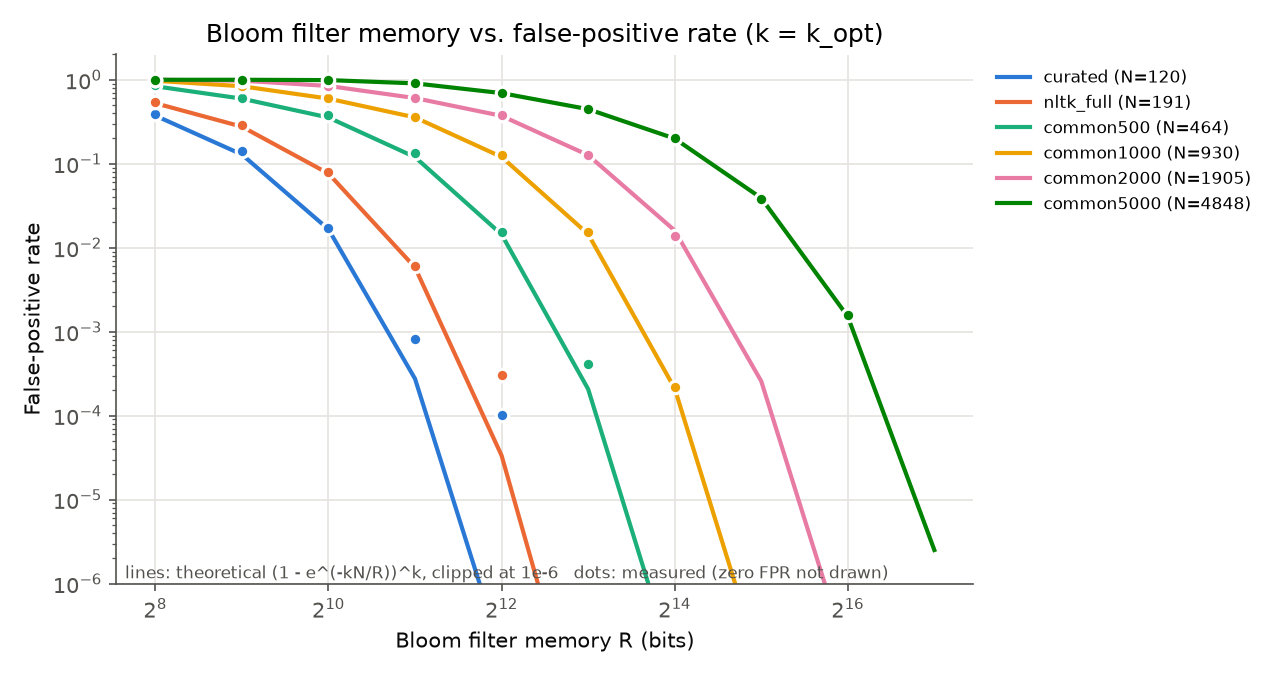
\includegraphics[width=\linewidth]{memory_vs_fpr.png}
  \caption{Bloom filter memory $R$ vs.\ false-positive rate, per vocabulary tier. Each curve falls
  as the filter grows; larger vocabularies need proportionally more bits, so their curves are
  shifted to the right.}
  \label{fig:memfpr}
\end{subfigure}\hfill
\begin{subfigure}{0.49\linewidth}
  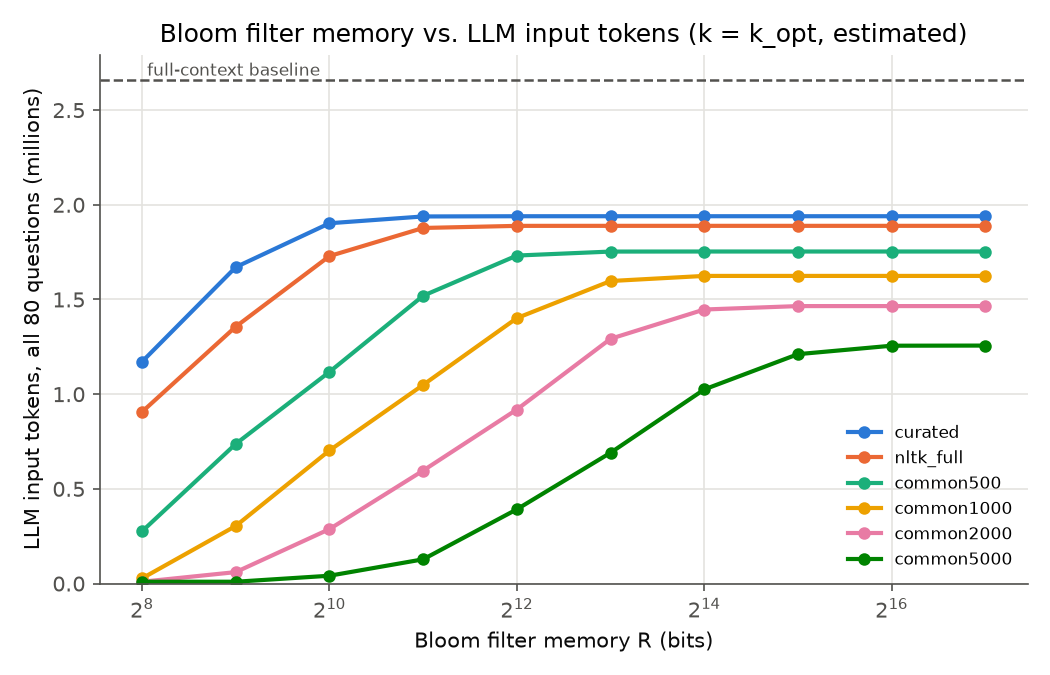
\includegraphics[width=\linewidth]{memory_vs_tokens.png}
  \caption{Bloom filter memory $R$ vs.\ total LLM input tokens over the 80 questions, per
  vocabulary tier (stats-only grid). Small filters have many false positives and delete extra
  words, so tokens are low; each curve flattens once the FPR is near zero, at a level set by the
  vocabulary alone.}
  \label{fig:memtok}
\end{subfigure}

\vspace{0.6em}
\begin{subfigure}{0.62\linewidth}
  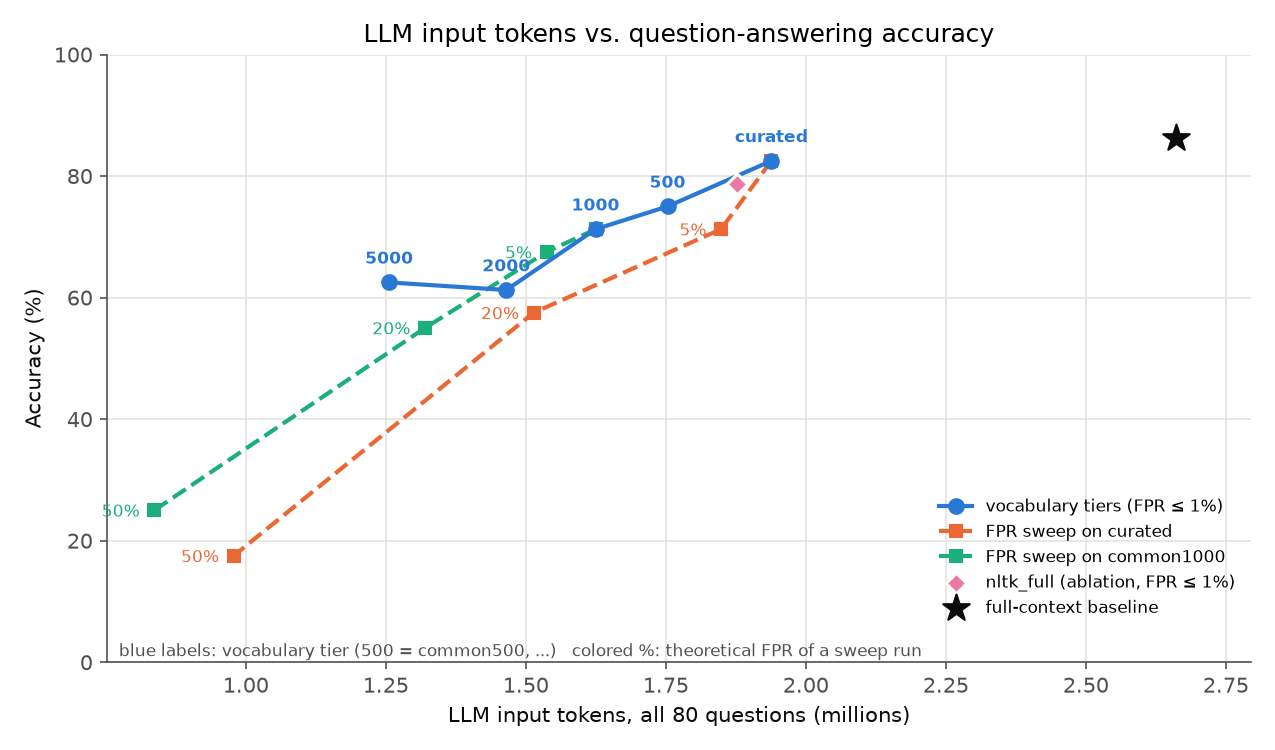
\includegraphics[width=\linewidth]{tokens_vs_accuracy.png}
  \caption{Total LLM input tokens vs.\ accuracy for all 13 LLM runs. The \code{nltk\_full}
  ablation uses the same filter size as \code{curated} ($R=2{,}048$, $k=7$), at a theoretical FPR
  of 0.58\% and a measured FPR of 0.62\%. Up and to the left is better (fewer tokens, higher
  accuracy); the blue tier line generally lies above the dashed FPR-sweep lines, so removing vocabulary
  words costs less accuracy per token saved than false positives do.}
  \label{fig:tokacc}
\end{subfigure}
\caption{How filter memory, false-positive rate, input tokens and accuracy trade off.}
\label{fig:tradeoffs}
\end{figure}

\begin{figure}[p]
\centering
\begin{subfigure}{0.49\linewidth}
  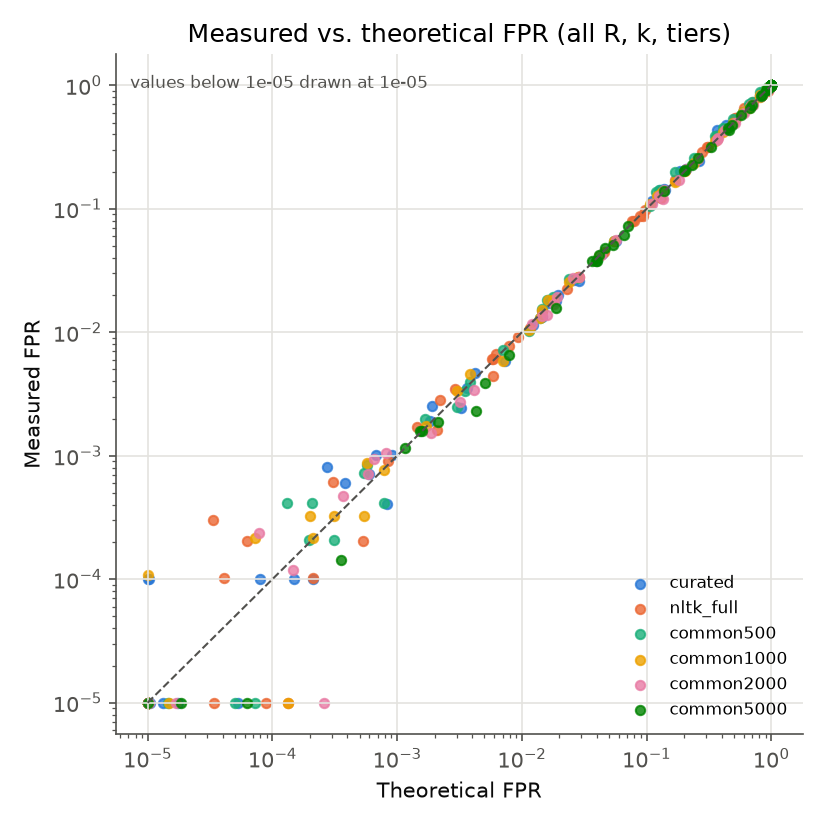
\includegraphics[width=\linewidth]{fpr_measured_vs_theory.png}
  \caption{Measured vs.\ theoretical FPR (stats-only grid). Points on the dashed $y=x$ line mean
  the filter behaves exactly as the formula predicts; the scatter at the bottom left comes from
  counting only a handful of false positives.}
  \label{fig:fprtheory}
\end{subfigure}\hfill
\begin{subfigure}{0.49\linewidth}
  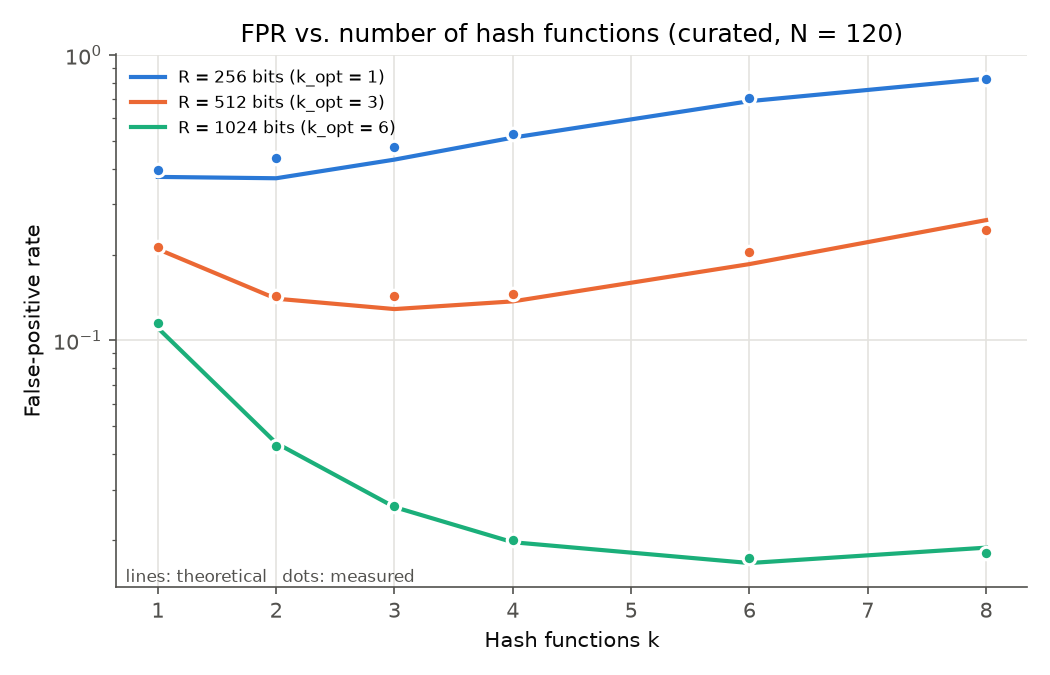
\includegraphics[width=\linewidth]{fpr_vs_k.png}
  \caption{FPR vs.\ $k$ at fixed $R$ (\code{curated}). Each curve has its minimum near
  $k_{\mathrm{opt}}$; for the smallest filter more hash functions only make the FPR worse, because
  they fill the bit array faster.}
  \label{fig:fprk}
\end{subfigure}

\vspace{0.6em}
\begin{subfigure}{0.49\linewidth}
  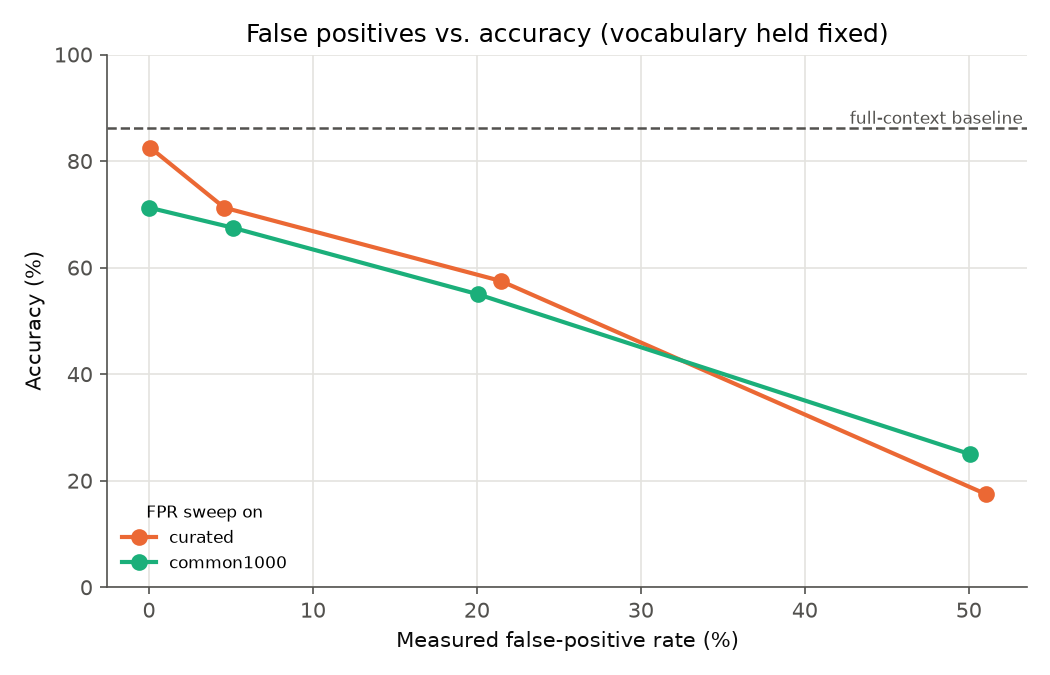
\includegraphics[width=\linewidth]{fpr_vs_accuracy.png}
  \caption{Measured FPR vs.\ accuracy, with the vocabulary held fixed. The steady downward slope
  shows that every extra false positive costs accuracy; the dashed line is the full-context
  baseline.}
  \label{fig:fpracc}
\end{subfigure}\hfill
\begin{subfigure}{0.49\linewidth}
  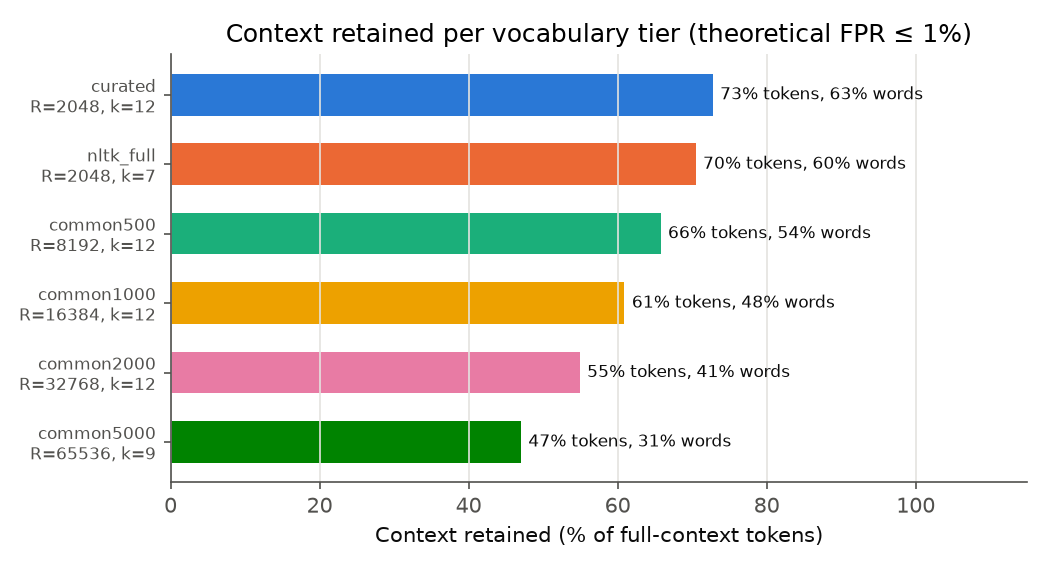
\includegraphics[width=\linewidth]{retained_by_tier.png}
  \caption{Context retained per tier, as a share of the full-context tokens (and words). Shorter
  bars mean more compression; tokens are always retained at a higher rate than words because the
  deleted words are cheap, short tokens.}
  \label{fig:retained}
\end{subfigure}
\caption{Filter behavior and the effect of false positives.}
\label{fig:filter}
\end{figure}

\begin{figure}[t]
\centering
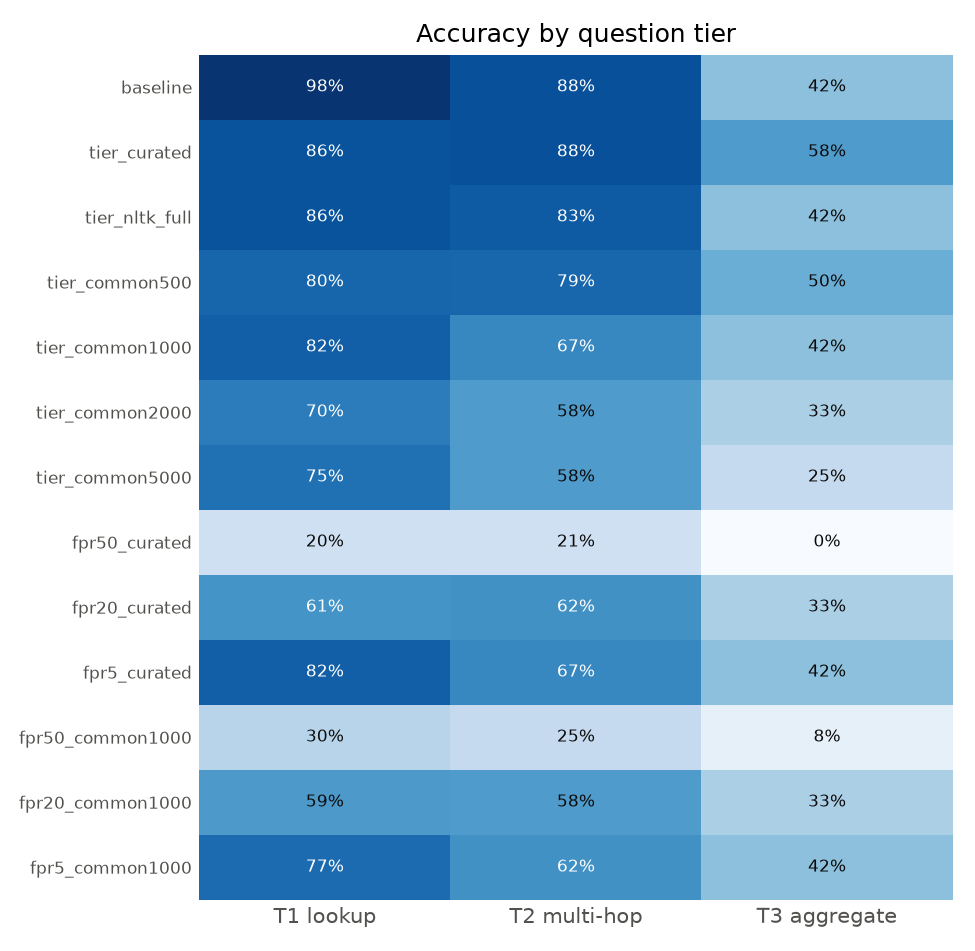
\includegraphics[width=0.7\linewidth]{accuracy_by_question_tier.png}
\caption{Accuracy by question tier for every run; darker cells are more accurate. Reading across
a row shows which kinds of questions a configuration hurts most, and the pale rows are the
high-FPR runs.}
\label{fig:breakdown}
\end{figure}

\clearpage
% =========================================================================== %
\section{Questions}
\label{sec:questions}
% =========================================================================== %

% --------------------------------------------------------------------------- %
\subsection{Q1: How does the measured false positive rate compare with the theoretical rate?}
% --------------------------------------------------------------------------- %
They agree closely, which confirms \textbf{H1}.
\begin{itemize}
  \item Across the stats-only grid, for every configuration whose theoretical FPR is at least 0.1\%,
        the measured FPR is within 4.4\% (relative) of $(1-e^{-kN/R})^k$ on average, and the points
        lie on the $y=x$ line (Figure~\ref{fig:fprtheory}).
  \item In the LLM runs, theory predicted 49.8\% / 20.2\% / 5.0\% for the \code{curated} sweep and we
        measured 51.0\% / 21.5\% / 4.6\%; for \code{common1000} the measured values were 50.1\% /
        20.1\% / 5.1\% against 50.0\% / 20.2\% / 5.0\% (Table~\ref{tab:summary}).
  \item Below about $10^{-4}$ the measurements scatter. There are only about 10{,}000 distinct
        non-member words in the four documents, so an FPR of $10^{-4}$ corresponds to roughly one
        false positive, and a single extra or missing hit moves the estimate a lot. For example,
        \code{tier\_curated} measured 0.08\% (8 words) against a theoretical 0.03\%, and
        \code{tier\_common2000} measured 0\%. These are counting noise, not a bias.
  \item The good agreement is expected from the hashing scheme: keyed BLAKE2b gives effectively
        uniform $h_1,h_2$, and Kirsch--Mitzenmacher double hashing is known to preserve the
        asymptotic FPR of $k$ independent hash functions.
\end{itemize}

% --------------------------------------------------------------------------- %
\subsection{\texorpdfstring{Q2: How do $R$ and $k$ affect}{Q2: How do R and k affect} the false positive rate and memory?}
% --------------------------------------------------------------------------- %
\begin{itemize}
  \item \textbf{Memory} is set by $R$ alone: exactly $R$ bits of payload, plus a constant of about
        600\,B of Python object overhead. $k$ does not change memory, only the number of bit
        positions computed per lookup.
  \item \textbf{$R$ (Figure~\ref{fig:memfpr}).} The FPR falls steeply as $R$ grows. What matters is
        the number of bits per word, $R/N$: the curves for larger vocabularies have the same shape,
        shifted right in proportion to $N$. To reach $\le 1\%$ FPR, \code{curated} ($N=120$) needs
        2{,}048 bits while \code{common5000} ($N=4{,}848$) needs 65{,}536. At $k_{\mathrm{opt}}$ every
        halving of the FPR costs a constant $\approx 1.44$ extra bits per word.
  \item \textbf{$k$ (Figure~\ref{fig:fprk}).} At a fixed $R$, FPR is minimized near
        $k_{\mathrm{opt}} = (R/N)\ln 2$. Two regimes are visible:
        \begin{itemize}
          \item \emph{Too few bits per word:} extra hash functions only fill the array faster. At
                $R=256$ for \code{curated} ($R/N\approx 2.1$, $k_{\mathrm{opt}}\approx 1.5$), the FPR
                rises from 0.37 at $k=1$ to 0.83 at $k=8$.
          \item \emph{Enough bits per word:} more hashes help, up to $k_{\mathrm{opt}}$; beyond it the
                FPR rises again slowly while lookups get slower. We cap $k$ at 16, past which the FPR
                is already negligible for our tiers.
        \end{itemize}
  \item \textbf{Compared with an exact set} (Table~\ref{tab:memory}), the filters are 16--48$\times$
        smaller, because they store bits instead of string objects and hash-table slots.
\end{itemize}

% --------------------------------------------------------------------------- %
\subsection{Q3: How do false positives affect the compressed context, token usage and accuracy?}
% --------------------------------------------------------------------------- %
A false positive deletes a word that should have stayed. Since every vocabulary word is removed
anyway, false positives only ever hit \emph{non-vocabulary} words: numbers, names, units, technical
terms. They lower token counts, but in the most damaging way possible, which confirms \textbf{H4}.
\begin{itemize}
  \item \textbf{Compressed context.} With \code{curated}, the 5\% / 20\% / 50\% FPR filters
        wrongly deleted 2{,}850 / 13{,}325 / 29{,}642 word occurrences (out of 90{,}772 words), vs.\ 37
        at 0.08\% FPR. Token-level retention falls from 72.7\% to 69.3\% / 56.7\% / 36.5\%.
  \item \textbf{Input tokens.} Total input tokens fall correspondingly, from 1.94M to 1.85M / 1.51M /
        0.98M for \code{curated} and from 1.62M to 1.54M / 1.32M / 0.84M for \code{common1000}.
  \item \textbf{Accuracy} falls roughly linearly with FPR (Figure~\ref{fig:fpracc}): 82.5\% $\to$
        71.3\% $\to$ 57.5\% $\to$ 17.5\% for \code{curated} and 71.3\% $\to$ 67.5\% $\to$ 55.0\% $\to$
        25.0\% for \code{common1000}. Even 5\% FPR already costs 11 points for \code{curated}, more than
        the whole difference between the baseline and \code{tier\_curated}.
  \item \textbf{False positives are a bad trade.} Figure~\ref{fig:tokacc} puts all runs on one
        axis. \code{fpr20\_curated} (1.51M tokens, 57.5\%) uses \emph{more} tokens than
        \code{tier\_common2000} (1.47M, 61.3\%) and is less accurate; \code{fpr50\_curated} uses 0.98M
        tokens for 17.5\%, while \code{tier\_common5000} uses 1.26M for 62.5\%. Removing words
        \emph{by design} buys far more compression per point of accuracy than removing them
        \emph{by accident}.
  \item \textbf{Conclusion.} False positives are pure loss. The filter should always be sized so the
        FPR is close to zero; compression should be tuned through the vocabulary, not through $R$.
\end{itemize}

% --------------------------------------------------------------------------- %
\subsection{Q4: How much can input tokens be reduced while staying close to the baseline?}
% --------------------------------------------------------------------------- %
\textbf{About 27\%.} \code{tier\_curated} reduces total input tokens from 2.661M to 1.938M (27.2\%)
at \textbf{82.5\% vs.\ 86.3\%} accuracy, i.e.\ 66 vs.\ 69 questions correct. Losing only three questions supports
\textbf{H3}.
\begin{itemize}
  \item \textbf{Cost.} At the paid-tier input price of \$0.30 per million tokens, the 80 baseline
        prompts cost \$0.80 and the \code{curated} prompts \$0.58, a saving of \$0.22 (27\%). Per
        question this is \$0.0100 vs.\ \$0.0073, so about \$2.70 saved per 1{,}000 questions on
        contexts of this size. Output tokens are negligible (about 400 per run in total, roughly \$0.001 at
        \$2.50 per million), so they do not change the comparison.
  \item \textbf{Tokens shrink less than words (H2 confirmed).} \code{curated} removes 37.2\% of
        words but only 27.3\% of context tokens. Function words are cheap single tokens; what
        survives (numbers, names, units, punctuation) costs several tokens per word. The saving also
        depends on the document: 33\% for the narrative \code{harbour} puzzle, 24\% for the
        number-dense \code{lunarleaper} paper (Table~\ref{tab:data}).
  \item \textbf{Question by question}, \code{curated} lost 8 questions that the baseline answered
        correctly and gained 5 that the baseline got wrong:
        \begin{itemize}
          \item \emph{Lost to grading, not to missing information} (3 of the 8 losses): the
                model copied the compressed wording, so the missing function words broke the exact
                match. It answered \code{berths 9 17} (gold: ``berths 9 through 17''),
                \code{150 1200 MHz} (gold: ``150 and 1200 MHz'') and
                \code{2 hours, 4 minutes 58 seconds} (the gold has ``and'').
          \item \emph{Lost to formatting:} two answers came back as \verb|$30^\circ$ to $40^\circ$|
                and \code{1-13 meters thick}.
          \item \emph{Lost to missing information} (3 of the 8): wrong berth counts on the
                \code{harbour} puzzle (\code{379 berths} instead of \code{9 berths}, \code{17 berths}
                instead of \code{16 berths}) and a wrong entity on \code{dwh} (\code{Corexit EC9527A}
                instead of \code{Port Bonython oil spill}).
          \item \emph{Gained} (5): questions the baseline got wrong. For example, the baseline answered
                \code{\$25 million} where \code{curated} gave the correct \code{\$45 million}, and
                \code{curated} gave the correct count of 5 where the baseline said 4. These gains most
                likely reflect the model's sensitivity to small input changes rather than a benefit of
                compression.
        \end{itemize}
  \item \textbf{By question type} (Table~\ref{tab:qtier}): lookup questions are hurt first
        (T1: 98\% $\to$ 86\%), while multi-hop accuracy is unchanged (88\%). T3 rises from 42\% to
        58\%, but with 12 questions that is two questions and should not be read as an improvement.
  \item \textbf{More aggressive tiers cost more accuracy.} \code{common500} saves 34\% of tokens at
        75.0\%, \code{common1000} 39\% at 71.3\%, and \code{common5000} 53\% at 62.5\%. Accuracy falls
        about 4 points per tier step up to \code{common1000}, drops sharply at \code{common2000}, and
        then levels off at about 61--63\%.
  \item \textbf{Fragile documents.} \code{harbour\_puzzle\_v1}, a logic puzzle with invented names
        and relations, is the most sensitive: it falls to 35\% at \code{common500}. Our hypothesis
        is that deleting common relational words scrambles who-is-what.
\end{itemize}

% --------------------------------------------------------------------------- %
\subsection{Q5: Is a larger Bloom filter always beneficial?}
% --------------------------------------------------------------------------- %
\textbf{No.} The answer depends on what the extra memory is used for.
\begin{itemize}
  \item \textbf{For a fixed vocabulary, extra memory stops helping almost immediately.} More bits
        lower the FPR, which restores wrongly deleted content words and raises accuracy, but once the
        FPR is near zero the compressed context no longer changes. The token curves in
        Figure~\ref{fig:memtok} level off at that point (\textbf{H5}). For \code{curated} this happens
        at about 2{,}048 bits (256\,B), where only 37 word occurrences out of 90{,}772 were deleted by
        false positives; doubling $R$ again could recover at most those.
  \item \textbf{Across vocabularies, more memory buys more compression but less accuracy.} A larger
        filter can hold a larger vocabulary at the same FPR, and a larger vocabulary deletes more
        tokens. Going from \code{curated} (2\,Kbit) to \code{common5000} (64\,Kbit) uses 32$\times$ the
        memory, cuts tokens kept from 73\% to 47\%, and drops accuracy from 82.5\% to 62.5\%.
  \item \textbf{The protected-word ablation} shows that the \emph{choice} of words matters more
        than their number. At the same 2{,}048 bits, \code{nltk\_full} (which also deletes negations,
        comparatives and unit letters) saves only 2 more points of tokens than \code{curated} (70.5\%
        vs.\ 72.7\% kept) but loses 3 more questions (78.8\% vs.\ 82.5\%).
  \item \textbf{Trade-off.} The best operating point is a small, carefully chosen vocabulary with
        just enough bits for FPR $\approx 0$, about 10--17 bits per word. Extra memory is only useful
        if the goal is more aggressive compression, and that costs accuracy. In every configuration
        the memory itself is tiny (at most 8.8\,KB) compared with an exact set (up to 375\,KB).
\end{itemize}

% --------------------------------------------------------------------------- %
\subsection{Q6: What are the limitations of using Bloom filters to compress context?}
% --------------------------------------------------------------------------- %
\begin{itemize}
  \item \textbf{The filter is blind to the question.} It removes the same words for every question.
        A word that is filler in general can be essential in one place, e.g.\ \emph{through} in
        ``berths 9 through 17''.
  \item \textbf{Word-level only.} It cannot drop redundant sentences or irrelevant sections, so the
        saving is capped by the share of tokens that are filler words: about 27\% for
        \code{curated}. Dense text (tables, numbers, technical papers) compresses least.
  \item \textbf{No sense of context.} A membership test cannot tell \emph{in} (preposition) from
        \emph{in} (inches), or \emph{US} from \emph{us}. The \code{common} tiers also delete short unit
        words such as \emph{ft} and \emph{km}. A natural extension of our work is to use domain-specific 
        vocabularies to mitigate this issue. 
  \item \textbf{False positives hit random words}, including possibly the answer itself. The filter
        must therefore be sized for FPR $\approx 0$. Its memory advantage over a set is real, but for a
        vocabulary of a few hundred words both are small, so the main benefit is a compact, fast,
        deterministic membership test rather than a necessary saving.
  \item \textbf{Telegraphic answers.} The model tends to copy the compressed wording into its
        answer, which hurts exact-match grading even when the information survived.
  \item \textbf{Language and tokenization.} The vocabulary is English-only and the method assumes
        whitespace-separated words.
\end{itemize}

% =========================================================================== %
\appendix
\section{Reproducibility}
% =========================================================================== %
\begin{itemize}
  \item \textbf{Command.} \code{README.md} gives the exact command: \code{experiments.py --mode all}
        with the four context, question and answer files passed explicitly. Without a cache it makes
        1{,}040 model calls, sends about 20.7M input tokens in total (about \$6 at \$0.30/M) and takes about 15 minutes; the paid compressed runs took 10\,min\,46\,s.
  \item \textbf{Determinism.} Hashing is keyed with seed 580; vocabularies are hard-coded or come from
        pinned \code{wordfreq} 3.1.1; generation uses temperature 0 and seed 580; all dependencies are
        pinned in \code{requirements.txt}.
  \item \textbf{Caching.} All responses and token counts are cached under \code{cache/}, so re-runs
        are free and reproduce the reported numbers exactly.
  \item \textbf{Tests.} 106 network-free unit tests (in \code{tests/}, not part of the submission)
        cover the filter, compression, prompt, grading and experiment code.
\end{itemize}

\end{document}
